\documentclass[UTF8,12pt]{ctexart}
\usepackage[a4paper,margin=2.4cm]{geometry}
\usepackage{graphicx}
\usepackage{booktabs}
\usepackage{longtable}
\usepackage{array}
\usepackage{enumitem}
\usepackage{xcolor}
\usepackage{float}
\usepackage{caption}
\usepackage{hyperref}
\usepackage{tikz}
\usetikzlibrary{arrows.meta,positioning,shapes.geometric,fit,calc}

\hypersetup{
  colorlinks=true,
  linkcolor=blue!55!black,
  urlcolor=blue!55!black
}

\graphicspath{{../screenshots/}}
\setlength{\parindent}{2em}
\setlength{\parskip}{0.35em}
\setlist{nosep,leftmargin=2em}
\renewcommand{\arraystretch}{1.25}
\captionsetup{font=small,labelfont=bf}
\sloppy

\definecolor{mainblue}{HTML}{1F5F99}
\definecolor{lightblue}{HTML}{EAF2FF}
\definecolor{linegray}{HTML}{CED6E0}
\definecolor{softyellow}{HTML}{FFF6DF}

\newcommand{\code}[1]{\texttt{\detokenize{#1}}}
\newcommand{\docmeta}[2]{\noindent\textbf{#1：}#2\par}
\newcommand{\screenshot}[3][0.8\textwidth]{
  \begin{figure}[H]
    \centering
    \includegraphics[width=#1]{#2}
    \caption{#3}
  \end{figure}
}

\tikzset{
  flow/.style={rectangle,rounded corners,draw=mainblue,fill=lightblue,minimum width=2.6cm,minimum height=0.9cm,align=center,font=\small},
  decision/.style={diamond,aspect=2,draw=mainblue,fill=softyellow,align=center,font=\small,inner sep=1pt},
  dataobj/.style={rectangle,draw=linegray,fill=white,minimum width=2.6cm,minimum height=0.85cm,align=center,font=\small},
  actor/.style={rectangle,rounded corners,draw=mainblue,fill=lightblue,minimum width=2.2cm,minimum height=0.9cm,align=center,font=\small\bfseries},
  usecase/.style={ellipse,draw=mainblue,fill=white,minimum width=2.9cm,minimum height=0.85cm,align=center,font=\small},
  classbox/.style={rectangle,draw=mainblue,fill=white,minimum width=3.1cm,minimum height=1.2cm,align=left,font=\small},
  arrow/.style={-{Latex[length=3mm]},thick,draw=mainblue},
  line/.style={thick,draw=mainblue}
}



\title{\textbf{基于 Python 的作业管理数据库应用系统设计说明书}}
\author{}
\date{}

\begin{document}
\maketitle

\docmeta{项目名称}{作业管理系统}
\docmeta{主要技术}{Python、Flask、SQLite、HTML/CSS}
\docmeta{系统类型}{数据库应用系统}

\section{系统概述}

本系统面向课程教学中的作业发布、学生提交和教师评分场景，目标是把传统手工收作业、统计提交情况、登记成绩等流程集中到一个 Web 系统中完成。系统采用浏览器访问方式，数据库使用 SQLite，本地即可运行，便于课程答辩和演示。

系统包含三类用户。管理员负责教师身份审核和基础数据管理；教师负责开设课程、布置作业、查看学生提交、下载附件、评分和导出统计；学生负责注册登录、加入课程、查看作业、提交或修改作业、查看成绩和评语。

系统设计重点体现面向对象思想。系统将用户、课程、作业、提交记录等现实对象抽象成数据库表和业务服务类，各类之间通过角色权限和外键关系形成清晰结构。页面层只处理表单和展示，业务逻辑集中在服务类中，数据库访问集中在数据库模块中。

\screenshot{02_admin_dashboard.png}{管理员后台界面}

\newpage

\section{需求分析与角色划分}

\subsection{管理员角色}

管理员是系统后台管理者，主要任务包括：

\begin{itemize}
  \item 查看系统用户、课程、作业和提交数量。
  \item 审核教师注册账号。
  \item 停用异常账号。
  \item 维护系统演示数据的整体可用状态。
\end{itemize}

管理员不直接参与课程教学业务，但对教师账号具有审核权限，防止普通用户直接获得教师功能。

\subsection{教师角色}

教师是课程和作业的创建者，主要任务包括：

\begin{itemize}
  \item 登录系统，创建课程并填写课程说明。
  \item 为自己的课程布置作业。
  \item 查看学生提交记录并下载学生上传文件。
  \item 对提交记录进行评分和填写评语。
  \item 导出作业提交统计 CSV 文件。
\end{itemize}

\subsection{学生角色}

学生是课程作业提交者，主要任务包括：

\begin{itemize}
  \item 注册并登录系统。
  \item 查看可选课程并加入课程。
  \item 查看自己已加入课程下的作业。
  \item 提交作业说明和附件。
  \item 在提交后再次修改作业。
  \item 查看教师评分和评语。
\end{itemize}

\newpage

\section{对象清单}

\begin{longtable}{>{\raggedright\arraybackslash}p{2.5cm}p{5.2cm}p{6cm}}
\toprule
对象 & 主要属性 & 主要功能 \\
\midrule
用户 & 用户名、密码哈希、姓名、角色、状态 & 注册、登录、权限判断、账号审核 \\
管理员 & 继承用户属性，角色为 admin & 审核教师、停用账号、查看统计 \\
教师 & 继承用户属性，角色为 teacher & 开课、布置作业、评分、导出 \\
学生 & 继承用户属性，角色为 student & 选课、提交作业、查看成绩 \\
课程 & 课程名称、课程说明、教师编号 & 保存课程信息，关联教师和学生 \\
选课记录 & 课程编号、学生编号 & 表示学生加入某门课程 \\
作业 & 作业标题、说明、截止时间、课程编号 & 保存教师发布的作业要求 \\
提交记录 & 作业编号、学生编号、文件名、说明、成绩、评语 & 保存学生提交内容和评分结果 \\
统计报表 & 作业名称、学生、提交时间、成绩 & 导出 CSV 文件，辅助教师统计 \\
\bottomrule
\end{longtable}

\begin{figure}[H]
\centering
\begin{tikzpicture}[node distance=1.25cm and 1.55cm]
  \node[dataobj,text width=2.55cm] (users) at (0,0) {USERS\\用户};
  \node[dataobj,text width=2.7cm] (courses) at (4.0,1.35) {COURSES\\课程};
  \node[dataobj,text width=2.7cm] (enrollments) at (4.0,-1.35) {ENROLLMENTS\\选课};
  \node[dataobj,text width=2.85cm] (assignments) at (8.2,1.35) {ASSIGNMENTS\\作业};
  \node[dataobj,text width=2.85cm] (submissions) at (8.2,-1.35) {SUBMISSIONS\\提交};

  \draw[arrow] (users.east) -- node[pos=0.52,above,fill=white,inner sep=1pt,font=\scriptsize]{教师开课} (courses.west);
  \draw[arrow] (users.east) -- node[pos=0.52,below,fill=white,inner sep=1pt,font=\scriptsize]{学生选课} (enrollments.west);
  \draw[arrow] (courses.east) -- node[above,fill=white,inner sep=1pt,font=\scriptsize]{发布作业} (assignments.west);
  \draw[arrow] (courses.south) -- node[right,fill=white,inner sep=1pt,font=\scriptsize]{课程成员} (enrollments.north);
  \draw[arrow] (assignments.south) -- node[right,fill=white,inner sep=1pt,font=\scriptsize]{作业提交} (submissions.north);
  \draw[arrow] (enrollments.east) -- node[below,fill=white,inner sep=1pt,font=\scriptsize]{学生记录} (submissions.west);
\end{tikzpicture}
\caption{数据库实体关系图}
\end{figure}

\newpage

\section{用例设计}

\begin{figure}[H]
\centering
\begin{tikzpicture}[
  uc/.style={ellipse,draw=mainblue,fill=white,minimum width=2.45cm,minimum height=0.72cm,align=center,font=\footnotesize},
  group/.style={draw=linegray,rounded corners,inner xsep=0.35cm,inner ysep=0.22cm}
]
  \node[actor] (admin) at (-5.2,2.3) {管理员};
  \node[uc] (a1) at (-1.8,2.75) {审核教师账号};
  \node[uc] (a2) at (1.35,2.75) {停用用户};
  \node[uc] (a3) at (-0.25,1.75) {查看基础统计};
  \node[group,fit=(a1)(a2)(a3)] (agroup) {};

  \node[actor] (teacher) at (-5.2,0.0) {教师};
  \node[uc] (t1) at (-1.8,0.5) {创建课程};
  \node[uc] (t2) at (1.35,0.5) {布置作业};
  \node[uc] (t3) at (-1.8,-0.5) {查看提交};
  \node[uc] (t4) at (1.35,-0.5) {评分导出};
  \node[group,fit=(t1)(t2)(t3)(t4)] (tgroup) {};

  \node[actor] (student) at (-5.2,-2.3) {学生};
  \node[uc] (s1) at (-1.8,-1.75) {加入课程};
  \node[uc] (s2) at (1.35,-1.75) {查看作业};
  \node[uc] (s3) at (-1.8,-2.75) {提交作业};
  \node[uc] (s4) at (1.35,-2.75) {查看成绩};
  \node[group,fit=(s1)(s2)(s3)(s4)] (sgroup) {};

  \node[draw=linegray,rounded corners,inner xsep=0.45cm,inner ysep=0.35cm,fit=(agroup)(tgroup)(sgroup)] (systembox) {};
  \node[font=\scriptsize,fill=white,inner sep=1pt] at (systembox.north) {系统功能};

  \draw[line] (admin.east) -- (agroup.west);
  \draw[line] (teacher.east) -- (tgroup.west);
  \draw[line] (student.east) -- (sgroup.west);
\end{tikzpicture}
\caption{系统用例图}
\end{figure}

\begin{longtable}{p{2.3cm}p{2.2cm}p{4.8cm}p{4.6cm}}
\toprule
用例 & 参与者 & 前置条件 & 结果 \\
\midrule
教师审核 & 管理员 & 教师已注册且状态为待审核 & 教师账号变为正常 \\
创建课程 & 教师 & 教师已登录且账号正常 & 数据库生成课程记录 \\
布置作业 & 教师 & 教师已创建课程 & 数据库生成作业记录 \\
提交作业 & 学生 & 学生已加入课程 & 数据库生成或更新提交记录 \\
作业评分 & 教师 & 学生已有提交记录 & 提交记录保存成绩和评语 \\
导出统计 & 教师 & 当前作业存在提交记录 & 浏览器下载 CSV 文件 \\
\bottomrule
\end{longtable}

\newpage

\section{类与模块设计}

系统主要业务类集中在 \code{assignment_system/services.py} 中。

\begin{longtable}{p{3.2cm}p{4.3cm}p{6.2cm}}
\toprule
类名 & 职责 & 关键方法 \\
\midrule
UserService & 处理注册、登录、账号状态 & register、authenticate、list\_users、set\_status \\
CourseService & 处理课程和选课 & create、list\_all、list\_by\_teacher、list\_by\_student、enroll \\
AssignmentService & 处理作业发布和查询 & create、get、list\_for\_teacher、list\_for\_student \\
SubmissionService & 处理提交、文件、评分 & save、list\_by\_assignment、get、grade、file\_path \\
ReportService & 处理统计导出 & assignment\_csv \\
\bottomrule
\end{longtable}

\begin{figure}[H]
\centering
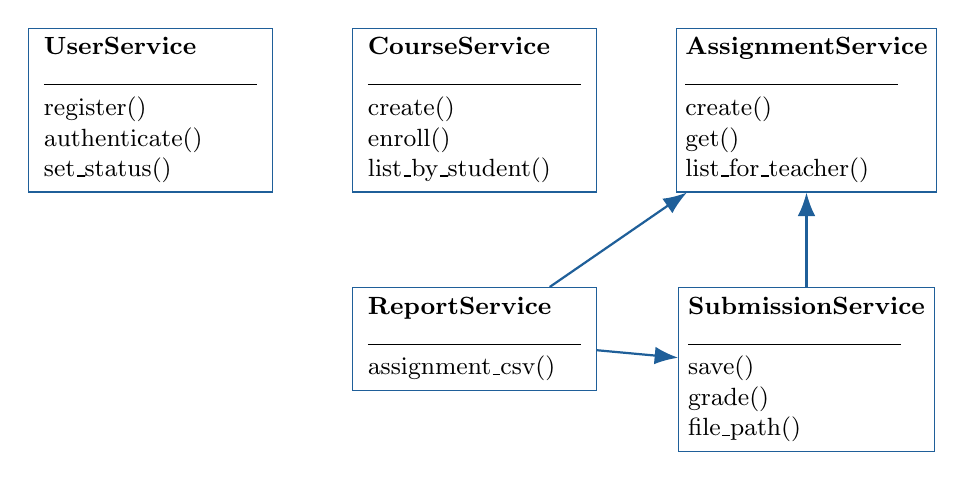
\begin{tikzpicture}[node distance=0.9cm and 1.0cm]
  \node[classbox] (user) {\textbf{UserService}\\\rule{2.7cm}{0.3pt}\\register()\\authenticate()\\set\_status()};
  \node[classbox, right=of user] (course) {\textbf{CourseService}\\\rule{2.7cm}{0.3pt}\\create()\\enroll()\\list\_by\_student()};
  \node[classbox, right=of course] (assign) {\textbf{AssignmentService}\\\rule{2.7cm}{0.3pt}\\create()\\get()\\list\_for\_teacher()};
  \node[classbox, below=1.2cm of assign] (submit) {\textbf{SubmissionService}\\\rule{2.7cm}{0.3pt}\\save()\\grade()\\file\_path()};
  \node[classbox, below=1.2cm of course] (report) {\textbf{ReportService}\\\rule{2.7cm}{0.3pt}\\assignment\_csv()};
  \draw[arrow] (report) -- (assign);
  \draw[arrow] (report) -- (submit);
  \draw[arrow] (submit) -- (assign);
\end{tikzpicture}
\caption{核心服务类关系图}
\end{figure}

\newpage

\section{数据库设计}

数据库采用 SQLite。SQLite 不需要单独安装数据库服务器，适合课程作业、单机演示和 Windows 答辩。数据库文件默认存放在 \code{data/assignment_system.sqlite3}。

\subsection{主要数据表}

\begin{longtable}{p{2.6cm}p{3cm}p{8cm}}
\toprule
数据表 & 作用 & 关键字段 \\
\midrule
users & 保存账号和角色状态 & id、username、password\_hash、name、role、status、created\_at \\
courses & 保存课程信息 & id、name、description、teacher\_id、created\_at \\
enrollments & 保存学生选课关系 & id、course\_id、student\_id、created\_at \\
assignments & 保存作业要求 & id、course\_id、title、description、deadline、created\_at \\
submissions & 保存提交和评分结果 & id、assignment\_id、student\_id、filename、content、score、comment \\
\bottomrule
\end{longtable}

\subsection{约束设计}

\begin{itemize}
  \item 用户名设置唯一约束，避免重复登录名。
  \item 角色字段限制为 admin、teacher、student。
  \item 教师账号注册后默认 pending，必须由管理员审核。
  \item 选课关系设置 course\_id 与 student\_id 联合唯一，避免重复选课。
  \item 提交记录设置 assignment\_id 与 student\_id 联合唯一，保证每个学生对同一作业只有一条当前提交记录。
\end{itemize}

\newpage

\section{主要流程设计}

\subsection{登录流程}

\begin{figure}[H]
\centering
\begin{tikzpicture}[node distance=1.15cm and 1.4cm]
  \node[flow] (start) {输入用户名\\和密码};
  \node[decision, below=of start] (exists) {账号\\存在?};
  \node[decision, below=of exists] (pwd) {密码\\正确?};
  \node[decision, below=of pwd] (status) {状态\\正常?};
  \node[flow, right=of exists] (err1) {提示登录失败};
  \node[flow, right=of status] (err2) {提示待审核\\或停用};
  \node[flow, below=of status] (ok) {进入对应\\工作台};
  \draw[arrow] (start) -- (exists);
  \draw[arrow] (exists) -- node[left]{是} (pwd);
  \draw[arrow] (exists) -- node[above]{否} (err1);
  \draw[arrow] (pwd) -- node[left]{是} (status);
  \draw[arrow] (pwd) -| node[pos=0.25,above]{否} (err1);
  \draw[arrow] (status) -- node[left]{是} (ok);
  \draw[arrow] (status) -- node[above]{否} (err2);
\end{tikzpicture}
\caption{登录判断流程图}
\end{figure}

\subsection{教师布置作业流程}

\begin{figure}[H]
\centering
\begin{tikzpicture}[node distance=1.0cm and 1.2cm]
  \node[flow] (a) {教师登录};
  \node[flow, right=of a] (b) {创建课程};
  \node[flow, right=of b] (c) {填写作业信息};
  \node[decision, below=of c] (d) {是否本人\\课程?};
  \node[flow, left=of d] (e) {拒绝操作};
  \node[flow, right=of d] (f) {保存作业};
  \node[flow, right=of f] (g) {学生端显示};
  \draw[arrow] (a) -- (b);
  \draw[arrow] (b) -- (c);
  \draw[arrow] (c) -- (d);
  \draw[arrow] (d) -- node[above]{否} (e);
  \draw[arrow] (d) -- node[above]{是} (f);
  \draw[arrow] (f) -- (g);
\end{tikzpicture}
\caption{教师布置作业流程图}
\end{figure}

\newpage

\section{学生提交与评分流程}

\begin{figure}[H]
\centering
\begin{tikzpicture}[node distance=0.9cm and 1.3cm]
  \node[flow] (a) {学生登录};
  \node[flow, below=of a] (b) {加入课程};
  \node[flow, below=of b] (c) {查看作业};
  \node[flow, below=of c] (d) {填写说明\\或上传文件};
  \node[decision, below=of d] (e) {已有\\提交?};
  \node[flow, below left=of e] (g) {新增提交};
  \node[flow, below right=of e] (f) {更新提交};
  \node[flow, below=1.35cm of e] (save) {保存提交记录};
  \node[flow, below=of save] (h) {教师查看};
  \node[flow, below=of h] (i) {评分评语};
  \node[flow, below=of i] (j) {学生查看成绩};
  \draw[arrow] (a) -- (b);
  \draw[arrow] (b) -- (c);
  \draw[arrow] (c) -- (d);
  \draw[arrow] (d) -- (e);
  \draw[arrow] (e) -- node[above left,font=\scriptsize]{否} (g);
  \draw[arrow] (e) -- node[above right,font=\scriptsize]{是} (f);
  \draw[arrow] (g.south) |- (save.west);
  \draw[arrow] (f.south) |- (save.east);
  \draw[arrow] (save) -- (h);
  \draw[arrow] (h) -- (i);
  \draw[arrow] (i) -- (j);
\end{tikzpicture}
\caption{学生提交与教师评分流程图}
\end{figure}

学生提交作业时，可以填写文字说明，也可以上传附件。教师评分后，成绩和评语保存在提交记录中，学生再次进入工作台即可查看。

\screenshot{05_student_submit.png}{学生提交作业页面}

\newpage

\section{前端界面设计}

系统前端采用简洁后台式布局，包括顶部导航、消息提示、表单面板、统计卡片、列表表格等组件。整体界面以白色和浅灰为主，按钮使用蓝色，便于区分主要操作。

\subsection{管理员界面}

管理员界面包含基础统计卡片和用户管理表格。教师账号待审核时，管理员可以点击“通过”按钮。

\screenshot{02_admin_dashboard.png}{管理员后台}

\subsection{教师界面}

教师界面分为课程创建、作业发布、课程列表、作业列表四部分，保证教师在一个工作台中完成主要操作。

\screenshot{03_teacher_dashboard.png}{教师工作台}

\newpage

\section{学生界面与提交界面}

学生界面分为“可选课程”和“我的作业”。学生加入课程后，课程下的作业会出现在作业列表中。

\screenshot{04_student_dashboard.png}{学生工作台}

教师查看提交后，可以填写成绩和评语，评分结果会保存到提交记录中。

\screenshot{08_teacher_after_grade.png}{教师评分后页面}

\newpage

\section{安全与运行设计}

\subsection{权限控制}

系统通过 session 保存登录用户编号，并在路由中使用角色权限检查。管理员页面只允许管理员访问，教师页面只允许教师访问，学生页面只允许学生访问。教师查看作业详情时，还会判断该作业是否属于当前教师。

\subsection{密码保存}

系统不直接保存明文密码，而是通过 Werkzeug 提供的哈希函数保存密码摘要。登录时通过哈希校验判断密码是否正确。

\subsection{文件上传}

学生上传文件时，系统会使用安全文件名处理，并在保存文件名前追加随机编号，避免不同学生上传同名文件时互相覆盖。

\subsection{Windows 兼容}

系统提供 \code{run_windows.bat} 一键运行脚本。脚本会创建虚拟环境、安装依赖、检查数据库并启动服务。数据库检查默认不会清空已有数据，只有手动执行 \code{python scripts/init_db.py --reset} 才会重置演示数据。

\subsection{打包设计}

系统提供 \code{build_windows_exe.bat} 和 GitHub Actions 工作流。Windows 环境可使用 PyInstaller 生成 \code{HomeworkSystem.exe}。源码运行是主方案，exe 是答辩备用方案。

\end{document}
